%%%%%%%%%%%%%%%%%%%%%%%%%%%%%%%%%%%%%%%%%%%%%%%%%%%%%%%%%%%%%%%%%%%%%%%%%%%%%%%%
%%
%%   BornAgain User Manual
%%
%%   homepage:   http://www.bornagainproject.org
%%
%%   copyright:  Forschungszentrum Jülich GmbH 2015
%%
%%   license:    Creative Commons CC-BY-SA
%%
%%   authors:    Scientific Computing Group at MLZ Garching
%%               C. Durniak, M. Ganeva, G. Pospelov, W. Van Herck, J. Wuttke
%%
%%%%%%%%%%%%%%%%%%%%%%%%%%%%%%%%%%%%%%%%%%%%%%%%%%%%%%%%%%%%%%%%%%%%%%%%%%%%%%%%

\chapter
%{GISAS and the DWBA}
{Grazing-incidence scattering and the distorted wave Born approximation}
  \label{SGisas}
\chaptermark{GISAS and the DWBA}

Wave propagation through thin layers requires
a special formalism that accounts for
refraction and reflection (\cref{Sfac21}).
Radiation impinging under grazing incidence
has long trajectories so that absorption is
often considerable (\cref{Sabsorption}).
The so obtained distorted plane waves are the base
for the reformulation of Born's scattering theory
in the distorted wave Born approximation (\cref{SDWBA}).
% TODO RESTORE XREF We also discuss the limits of coherent superposition (\cref{Scoherlen}),

%%%%%%%%%%%%%%%%%%%%%%%%%%%%%%%%%%%%%%%%%%%%%%%%%%%%%%%%%%%%%%%%%%%%%%%%%%%%%%%%
\section[Wave propagation in $2+1$ dimensions]{Wave propagation in $\v{2+1}$ dimensions}\label{Swave21}
%%%%%%%%%%%%%%%%%%%%%%%%%%%%%%%%%%%%%%%%%%%%%%%%%%%%%%%%%%%%%%%%%%%%%%%%%%%%%%%%

\begin{figure}[tb]
  \centering
    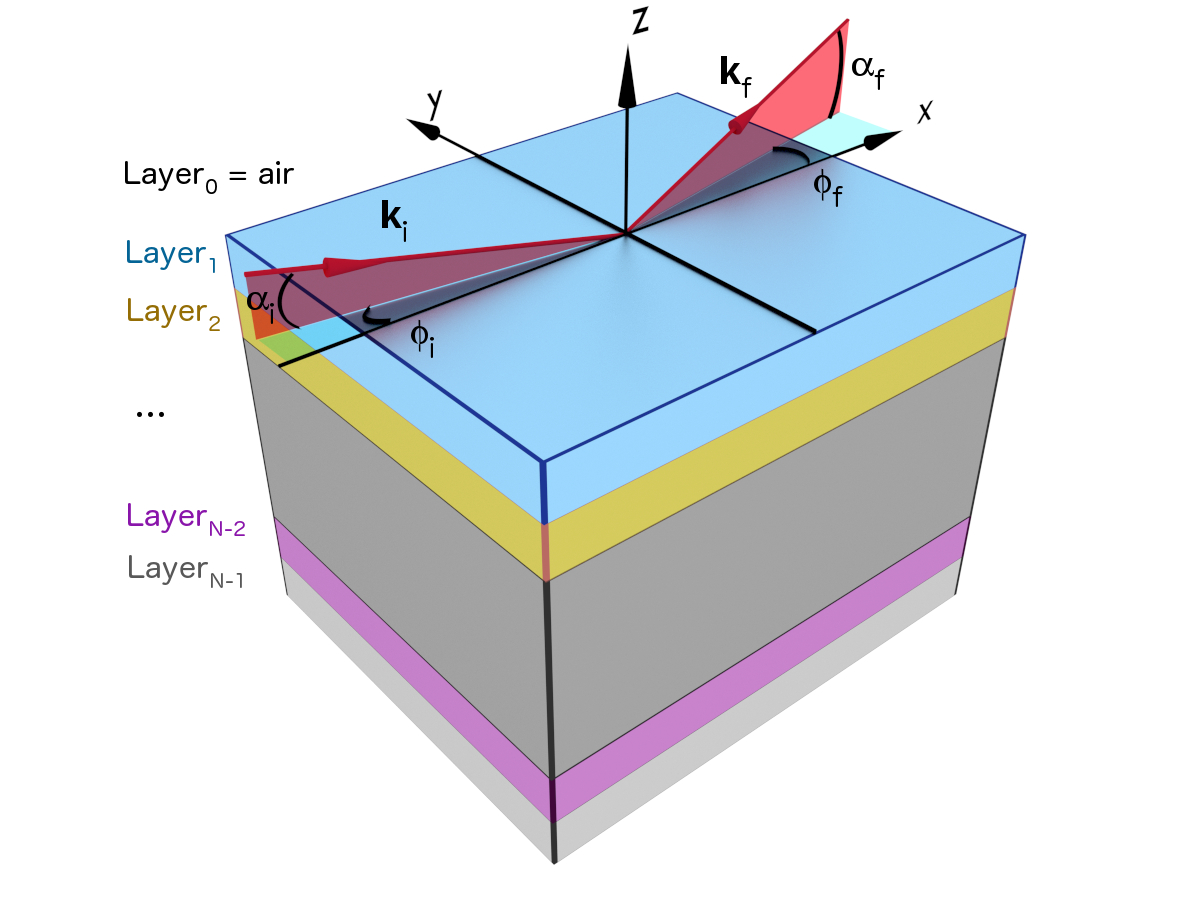
\includegraphics[clip=, width=120mm]{fig/drawing/setup_multilayer.jpg}
  \caption[Conventional GISAS scattering geometry.]{Geometric conventions
  in GISAS scattering comprise a Cartesian coordinate system
  and a set of angles.
  The coordinate system has a $z$ axis normal to the sample plane,
  and pointing into the halfspace where the beam comes from.
  The $x$ axis usually points along the incident beam,
  projected onto the sample plane.
  Incident and final plane waves are characterized
  by wavevectors $\k_\ti$, $\k_\tf$;
  the angle $\alpha_\ti$ is the incident glancing angle;
  $\phi_\ti$ is usually zero, unless used to describe a sample rotation;
  $\alpha_\tf$ is the exit angle with respect to the sample's surface;
  and $\phi_\tf$ is the scattering angle with respect to the scattering plane.
  In the above figure $\phi_\tf$ is negative by convention, while all other angles
  are positive.
\nomenclature[1α024 2i000]{$\alpha_\ti$}{Glancing angle of the incident beam}
\nomenclature[1α024 2f000]{$\alpha_\tf$}{Glancing angle of the detected beam}
\nomenclature[1φ024 2i000]{$\phi_\ti$}{Angle between the incident beam, projected into the sample plane, and the $x$ axis}%
\nomenclature[1φ024 2f000]{$\phi_\tf$}{Angle between the detected beam, projected into the sample plane, and the $x$ axis}%
\nomenclature[2x020]{$x$}{Horizontal coordinate, usually chosen along the incoming beam projection}%
\nomenclature[2y020]{$y$}{Horizontal oordinate, chosen normal to $z$ and $x$}%
  The numbered layers illustrate a multilayer system as dicussed in \cref{sec:Multilayers}.
\index{Layer!numbering}%
\index{Multilayer}
  }
  \label{fig:expgeom}
\end{figure}

Reflectometry and grazing-incidence scattering
are designed for the investigation of surfaces, interfaces, and thin layers,
or most generically:
samples with a $2+1$ dimensional structure
that are on average translationally invariant in $x$ and $y$ direction,
but structured in $z$ direction.
\nomenclature[2x020]{$x$}{Horizontal coordinate, in the sample plane}%
\nomenclature[2y020]{$y$}{Horizontal coordinate, in the sample plane}%
\nomenclature[2z020]{$z$}{Vertical coordinate, along the sample normal}%
By convention,
we designate the \E{sample plane} ($xy$) as \E{horizontal},
\index{Sample plane}%
\index{Horizontal plane}%
and the \E{sample normal} ($z$) as \E{vertical},
\index{Sample normal}%
\index{Vertical direction}%
\index{Conventions|see {Horizontal and Vertical}}%
even if this does not correspond to the actual experimental geometry.\footnote
{In many reflectometers,
 the scattering plane and the sample normal are horizontal in laboratory space.}
The $z$ axis points upwards, hence out of the sample towards the
vacuum (or air) halfspace where the incident radiation comes from,
as illustrated in \cref{fig:expgeom}.
% TODO: add figure

Vertical modulations of the refractive index $n(z)$
cause refraction and reflection of an incident plane wave.
\index{Glancing angle}%
\index{Refraction}%
\index{Reflection}%
For small glancing angles,
these distortions can be arbitrary large,
up to the limiting case of total reflection,
even though $1-n$ is only of the order $10^{-5}$ or smaller.
Such zeroth-order effects cannot be accounted for
by perturbative scattering theory.
Instead, we need to deal with refraction and reflection
from the onset, in the wave propagation equation.

Therefore we have to modify our derivation of
the scattering cross section~\cref{Exsection} at an early stage,
namely at the decomposition~\cref{Edecompose_v} of the scattering length density.
\index{Scattering length density}%
We replace~\cref{Edecompose_v} by
\begin{equation}\label{Edecompose_vz}
  v(\r) = \overline{v}(z) + \delta v(\r),
\end{equation}
allowing for vertical variations of~$\overline{v}$.
Equations~\cref{Edispersion} and \cref{EnRefrIndx} must be modified
to allow for a $z$~dependence of the refractive index~$n(z)$ and the wavenumber~$K(z)$.
The homogeneous wave equation~\cref{EHelmholtzHomog} takes the form
\begin{equation}\label{EHelmholtzGradedHomog}
  \left\{\Nabla^2+K(z)^2\right\}\psi(\r) = 0.
\end{equation}
It is solved for the horizontal coordinate~$\r_\parallel$
by the factorization ansatz
\Emph{
\begin{equation}\label{Ekpar}
\psi(\r) = \e^{i \k_\parallel\r_\parallel} \phi(z).
\end{equation}\vspace*{-10pt}
}
\nomenclature[2k041\parallel]{$\k_\parallel$}{Projection of $\k$ onto the sample plane}%
\nomenclature[1φ020 0z020]{$\phi(z)$}{$z$-dependent factor of $\psi(\r)$}%
The horizontal wavevector $\k_\parallel$ remains constant
as initialized by the incoming beam.
The factorization ansatz \cref{Ekpar} leaves us some freedom
how to deal with an imaginary part of~$n$.
We \E{choose} that horizontal wavevectors~$\k_\parallel$
shall always be real.
The damping then appears in the vertical wavefunction~$\phi(z)$
that is governed by the one-dimensional wave equation
\Emph{
\begin{equation}\label{Ewavez}
\left\{\partial_z^2 + K(z)^2 - k_\parallel^2 \right\} \phi(z) = 0.
\end{equation}\vspace*{-10pt}
}
This equation has no practicable solution for arbitrary functions~$K(z)$.
In BornAgain, samples are assumed to consist of a finite number of discrete layers.
\index{Multilayer!refractive index profiles}%
\index{Layer!refractive index profiles}%
Within one layer, the refractive index must either be constant,
or have an affine linear dependence $n(z)^2=a+bz$.
All other cases must be handled by dividing the sample into many layers
and approximating $n(z)^2$ by a step function.

\Work{Support for linear gradings with $n(z)^2=a+bz$ is not yet implemented.}
\index{Refractive index!graded}%
\index{Graded layer}%
\index{Layer!graded}%
\iffalse
For a graded refractive index~$n$
 that is a smooth function of~$z$,
the differential equation~\cref{Ewavez} is best solved
using the WKB method.\footnote
{Also called \E{semiclassical approximation} or
\E{phase integral method},
%originally developed
%by Liouville (1837), Green (1837), Lord Rayleigh (1912), and Jeffreys (1923),
named after Wentzel (1926), Kramers (1926), Brillouin (1926).
See any textbook on quantum mechanics.}
\index{WKB method}%
\index{Semiclassical approximation|see {WKB method}}%
\index{Phase integral method|see {WKB method}}%
\fi

When an incident plane wave,
travelling downwards with
$\phi(z)=\e^{-ik_\perp z}$,
\nomenclature[2k021\perp]{$k_\perp$}{Component of $\k$ along the sample normal}%
impinges on a sample with $n(z)\ne 1$,
then the wave is partly reflected ($-k_\perp$ reversed into $+k_\perp$)
and partly refracted
($k_\perp$ changing while $\k_\parallel$ stays constant,
resulting in a change of glancing angle).
Similarly, reflection and refraction occur
whereever $n(z)$~varies.
As a result, throughout the vertical wavefunction $\phi(z)$ is composed of a
downward travelling component $\phi^-(z)$
and an upward travelling component $\phi^+(z)$.
The only exception is in the homogeneous substrate at the bottom of the sample,
where there is no incoming upward travelling wave.

For a stepwise refractive index profile,
the $\phi^\pm(z)$ are derived from continuity conditions at the layer interfaces.
The limiting values on approaching the interface from above or below
are related to each other through Fresnel's
transmission and reflection coefficients.
\index{Fresnel coefficients}%
This will be elaborated in \Cref{Sacrolay}.

The following derivations in \Cref{SDWBA}, however,
are not restricted to specific refractive index profiles.
They hold for whatever solutions
$\psi^\pm(\r)$ of the wave equation~\cref{EHelmholtzGradedHomog}.


\index{Absorption|)}%

%===============================================================================
\section{Distorted-wave Born approximation (DWBA)}\label{SDWBA}
%===============================================================================

\index{Distorted-wave Born approximation|(}%
\index{DWBA|see {Distorted-wave Born approximation}}%

The standard form of the Born approximation,
as presented in \cref{SBornApprox},
combines an approximation scheme
(computing \cref{EPsiFormal} by iteration)
with an assumption (the incident field is a plane wave)
and an analytic result
(in far-field approximation,
the Green function of the Helmholtz equation is a plane wave
with respect to the locus of scattering).
These three elements must not necessarily go together.
We can apply the very same approximation scheme,
even if the incident field is not a plane wave,
but a \E{distorted wave},
namely a superposition of downwards and upwards travelling plane waves,
as derived in the previous section.
This is the core idea
of the \E{distorted-wave Born approximation} (DWBA).\footnote
{The distorted-wave Born approximation
was originally devised by Massey and Mott (ca 1933)
for collisions of charged particles.}
% Schiff (^3 1968, p 327) cites
% Mott, Massey, The Theory of Atomic Collisions, p 100, Oxford 1933;
% There are also several papers by Massey and Mott from about 1933.

To carry out this idea, we need to determine the Green function~$G$.
\index{Green function!vertically structured material}%
In \cref{SBornExpans} we did so quite specifically
for a homogeneous material.
Computing~$G$ in closed form for a more generic wave equation
like~\cref{EHelmholtzGradedHomog} is far more difficult,
if not outright impossible.
Fortunately, this computation is not necessary,
and would be but wasted effort:
We do not need the full solution~$G(\r,\r')$,
but only its asymptotic far-field value $G(\rD,\r')$
at a detector position $\rD$.
\nomenclature[2r041 2d100]{$\rD$}{Position of the detector}%
Thanks to a \E{source-detector reciprocity theorem}~\cref{Ereci}
\index{Reciprocity}%
proven in \cref{Sreci1},
we can compute this value
as
\begin{equation}\label{EreciDup}
  G(\rD,\r) = B(\r,\rD),
\end{equation}
\nomenclature[2b030 2r040 2r041]{$B(\r,\r')$}{Green function, adjoint of $G$}%
where~$B$ is the \E{adjoint Green function}
that describes backward propagation from $\rD$ into the sample.

Outside the sample,
$B$ obeys the Helmholtz equation
with isolated inhomogeneity \cref{EHelmholtzForGreen},
and therefore has the far-field expansion~\cref{EGreenFar},
\index{Far-field approximation}%
\begin{equation}\label{EBFar}
  B_\text{far}(\r,\rD)
  =\frac{\e^{iKr_\text{D}}}{4\pi r_\text{D}}\e^{-i\k_\tf \r}.
\end{equation}
When this backward propagating plane waves impinges on the sample,
it undergoes reflection and refraction in exactly the same way as
the incident plane wave $\e^{i\k_\ti\r}$.
Therefore,
 \cref{EBFar} admits a generalization that also holds inside the sample:
\begin{equation}\label{EBFull}
  B_\text{far}(\r,\rD)
  = \frac{\e^{iKr_\text{D}}}{4\pi r_\text{D}}\psi^*_\tf(\r).
\end{equation}
Applying now the reciprocity theorem \cref{EreciDup},
we obtain
\begin{equation}\label{EGreenFarDWBA}
  G_\text{far}(\r,\r')
  = \frac{\e^{iKr}}{4\pi r}\psi^*_\tf(\r')
\end{equation}
which agrees literally with \cref{EGreenFar},
though $\psi_\tf$ is not any longer a plane wave.
Accordingly,
the scattered far-field is still given by \cref{EsandwichC},
and the differential cross section by \cref{Exsection}.
We only need to redetermine the matrix element
$\bra \psi_\ti|\delta v|\psi_\tf\ket$,
which no longer has the plane-wave form~\cref{Echiq}.

Since both the incident
and the scattered distorted wavefunction
are composed of downward and upward propagating waves,
\begin{equation}\label{Epsipm}
  \psi_w(\r)
  = \psi^-_w(\r) + \psi^+_w(\r)
  \quad\text{with}\quad
  w=\ti,\tf,
\end{equation}
\nomenclature[2w010]{$w$}{An index that can take the values i (incident)
or f (final)}%
the matrix element can be expanded into four terms,
\begin{equation}\label{Edwba4}
  \bra \psi_\ti|\delta v|\psi_\tf\ket
  = \bra \psi^-_\ti|\delta v|\psi^-_\tf\ket
  + \bra \psi^-_\ti|\delta v|\psi^+_\tf\ket
  + \bra \psi^+_\ti|\delta v|\psi^-_\tf\ket
  + \bra \psi^+_\ti|\delta v|\psi^+_\tf\ket,
\end{equation}
\nomenclature[1ψ041 0\pm 2r040]{$\psi^\pm(\r)$}{Upward ($+$) or downward ($-$) propagating component of $\psi(\r)$}%
\nomenclature[0\pm]{$\pm$}{Upward ($+$) or downward ($-$) propagating}%
or in an obvious shorthand notation
\Emph{%
\begin{equation}\label{Edwba}
  \bra \psi_\ti|\delta v|\psi_\tf\ket
  = \sum_{\pm_\ti} \sum_{\pm_\tf}
    \bra \psi^\pm_\ti|\delta v|\psi^\pm_\tf\ket.
\end{equation}%
\vspace*{-5pt}}
This equation contains the essence of
the distorted-wave Born approximation
for small-angle scattering under grazing incidence,
and is the base for all scattering models implemented in \BornAgain.
Since $\bra \psi_\ti|\delta v|\psi_\tf\ket$
appears as a squared modulus
in the differential cross section~\cref{Exsection},
the four terms of \cref{Edwba} can interfere with each other,
which adds to the complexity of GISAS patterns.

\index{Distorted-wave Born approximation|)}%


%%%%%%%%%%%%%%%%%%%%%%%%%%%%%%%%%%%%%%%%%%%%%%%%%%%%%%%%%%%%%%%%%%%%%%%%%%%%%%%%
%\iffalse
\section{Coherence length [TO REVISE]}\label{Scoherlen}
%%%%%%%%%%%%%%%%%%%%%%%%%%%%%%%%%%%%%%%%%%%%%%%%%%%%%%%%%%%%%%%%%%%%%%%%%%%%%%%%

\index{Coherence length|(}%
The matrix elements $\bra \psi^\pm_\ti|\delta v|\psi^\pm_\tf\ket$
are given by three-dimensional integrals~\cref{Etrama},
\begin{equation}\label{Etrama3}
  \bra \psi_\ti^\pm|\delta v|\psi_\tf^\pm\ket
  \coloneqq  \int\!\d^3r\, \psi^{\pm*}_\ti(\r)\delta v(\r)\psi^\pm_\tf(\r).
\end{equation}
The integration domain is effectively limited to a finite $z$ interval,
where $\delta v(\r)$ is horizontally modulated.
On the other hand, the horizontal integration domain is infinite
within our formalism,
which is of course an idealization.
Obviously, physical integration limits are imposed by the finite
\E{illuminated sample area}.\footnote
{For a given instrument setup,
the incoming beam illuminates a finite area~$A_\ti$ in the sample plane,
and similarly, scattered radiation is only detected if it originates
from an area~$A_\tf$ that can be determined
by tracing back rays from the detector
to their intersection with the sample plane.
In a well aligned instrument, $A_\ti$ and $A_\tf$ are nearly the same.
Let $A_\text{beam}\coloneqq A_\ti\cap A_\tf$.
In a well aligned experiment,
$A_\text{beam}$ is equal to or a subset of $A_\text{sample}$
(if $A_\ti$ or $A_\tf$ are larger than $A_\text{sample}$,
collimation slits should be narrowed
lest useless rays cause avoidable noise).
Anyhow, the horizontal integration domain
is limited to the \E{illuminated sample area} (``beam footprint'')
$A_{xy}\coloneqq A_\text{sample}\cap A_\text{beam}$.}
\index{Sample area}%
\index{Illumination!beam footprint on sample}%
\index{Beam footprint}%
Another limitation comes from the finite \E{coherence length}
of the instrumental setup,
which usually is much shorter than the sample width and length
%This is of importance in neutron scattering
%where typical sample dimensions of 1\ldots10~mm
%are much larger than the relevant coherence length,
%which is of the order 10\ldots100~$\upmu$m
\cite{HaPR10,MaMM14}.\footnote
{These two references also make clear that
  the theoretical description and the experimental determination of
  coherence lengths are difficult problems and subject of ongoing research.}

While each single neutron is described by a wavefunction
that allows for \E{coherent} superposition of
different contributions to the scattered wavefunction,
the final detector statistics
\index{Detector statistics}%
is given by an \E{incoherent} sum
over the differential cross sections of individual neutrons.
The finite \E{resolution}
\index{Resolution|(}%
of an experimental setup is in part due to the fact that
different neutrons have different wavenumbers,
originate\footnote
{It is reasonable to take the last collision in the moderator
  as the \E{origin} of a neutron ray,
  since collisions between neutrons and hydrogen nuclei bound in
  disordered matter lead to almost perfect decoherence.}
at different points in the moderator,
and are detected at slightly different points within one detector pixel.
This can be modeled by computing expected scattering intensities as
averages over different neutrons with
$K$, $\v{\hat k}_\ti$, and $\v{\hat k}_\tf$ drawn at random
from appropriate distributions.
% TODO RESTORE TEMPORARILY REMOVED XREF as described in \cref{Sresolution}.

However, this is not the full story.
In the above introduction to the Born approximation
we have made the standard assumption
that an incoming neutron can be described by a plane wave
$\psi_\ti=\e^{i\k_\ti\r}$.
The wavefunction $\psi_\tf$ traced back from the detector is also
approximated by a plane wave.
In the DWBA we allow these waves to be distorted within the sample,
but when impinging on the sample they still are plane.
A plane wave obviously is an idealized concept,
since it has infinite lateral extension.
The \E{transverse coherence length} indicates the scale
beyond which this approximation becomes invalid.
At larger scales, the wave fronts appear randomly distorted.
Physical causes of these distortions include
reflections in the neutron guide,
diffraction by guide windows and other slits,
and diffraction by imperfect monochromator crystals.
Of course the distorted wave still admits a Fourier decomposition
into plane waves with slightly different wavevectors.
In practice, it is impossible to distinguish this spread of wavevectors
from the incoherent spread described in the previous paragraph.
The instrumental resolution function therefore
accounts for both causes of wavevector distortion.
\index{Resolution|)}%

Usually, therefore, a GISANS image is an incoherent average
over coherent diffraction patterns collected from
many small subareas of the sample.
Only horizontal sample structures on scales smaller the coherence length
yield interference patterns.
Structure fluctuations on larger scales
produce said incoherent average of different GISANS images.

The crossover from coherent to incoherent scattering is of course
a gradual one.
The coherence length, however defined,
indicates where a certain, somewhat arbitrary degree
of decoherence is reached.
Under these reservations
one defines a \E{coherence spot}
in the cross section of an approximately plane wave
as an area where the coherence is above a certain threshold.
Unless the wave has been prepared in a highly anisotropic guide and slit system,
this spot is about circular.
Under grazing incidence conditions however,
the projection of this spot onto the sample surface
yields a very elongated ellipse.
Therefore, the coherence length is much larger in $x$ than
in $y$ or $z$ direction.\footnote
{This has nothing to do with the distinction of
  \E{transverse} and \E{longitudinal} coherence length.
  Longitudinal coherence has to do with wavelength stability
  and is of no importance for elastic scattering.
  We are talking here about \E{horizontal} and \E{vertical}
  projections of the \E{transverse} coherence length.}

\Note{\indent Unless otherwise said, \BornAgain\ simulates
  \E{coherent} diffraction patterns obtained by
  the linear superposition of scattered waves.
  To simulate an \E{incoherent} mixture of diffraction patterns,
  the most generic solution is a script with an outer loop
  that averages over several coherent computations with
  appropriately distributed parameters.}

% TODO: more about implementation !

\index{Coherence length|)}%
%\fi
